\chapter{How to operate}



One day  $+$ means to add natural numbers, the next day 
polynomials, later matrices.  
You can even add colors ``Yellow=Blue+Green''. When you program 
you learn to add strings
\begin{center}
\begin{notebookin}
print "Algebra " + " is " + " computation"
\end{notebookin}
\begin{notebookout}
Algebra is computation
\end{notebookout}
\end{center}
If we focus on our 
speech we find more expansive uses:
``add the flour, water, yeast, and salt'' or  
``count each household, then add''.  

These suggest that addition is a stand in, a variable.  It is not however 
an ordinary variable.  We don't replace $+$ sign with a numbers.  
Addition depends on some inputs, the total 
number being its \emph{valence}.    It also depends on a grammar.
It may be \emph{infix} $2+3$ as we commonly 
use with arithmetic.  It can be \emph{prefix} $+,2,3$ as in the recipe instructions,
or it could be \emph{postfix} $2,3,+$; as in the census illustration.  
The variations in grammar are like any language 
where there could be a dialect that evolves the operator's grammar and lexicon.
 HP calculators were postfix for some time to match engineering requirements.
A program to add two lists could get away with the following linguistic drift:
\begin{center}
\begin{notebookin}
cat [3,1,4] [1,5,9]
[3,1,4] + [1,5,9]
\end{notebookin}
\begin{notebookout}[2]
[3,1,4,1,5,9]
[4,6,13]
\end{notebookout}
\end{center}
Using \texttt{cat} reminded us to concatenate and avoided confusion with the
later $+$ concept.  It was the better choice. Challenge yourself to see both as
addition and you will find addition everywhere. 

Addition  may be with two or more terms.  It also may be 
sensitive to order: ``add the food coloring to the vinegar, then add the baking
powder'' is a different to ``add the vinegar and baking powder than the
food coloring''.  To make a manageable theory, algebra needs fewer variations that 
build towards this complexity.



\section{Fixed Valence Operators}
While programming languages have entertained the possibility of 
variable valence for operators (look into \emph{variadic} evaluation)
by far the most common approach in scientific abstraction of operators 
is to study those with a fixed valence.  Often by composing several 
operators in a row we obtain the same effect a  variadic 
operator.  Addition from here on out will be bivalent, meaning 
requiring 2 inputs, and with infix grammar $\Box +\Box$.


Since we are evolving, we may as well permit multiplication as a bivalent (binary) operator
symbol, changing the signature to $\Box \cdot \Box$, i.e. $2\cdot 4$; or
$\Box\Box$, e.g. $xy$.   Avoid $\Box\times \Box$, we need that symbol elsewhere.
These days composition $\Box\circ\Box$ is written as multiplication; so, you can
use that symbol however you like.  Addition is held to high standards in algebra
(that it will evolve into linear algebra).  So when you are considering a binary
operation with few if any good properties, use a multiplication inspired
notation instead.   





Valence 1, \emph{unary} (univalent), operators include the negative sign $-\Box$ to create 
$-2$.  The transpose of a matrix is a unary operator.  Programming languages add several others 
such as \lstinline{++i, --i} which are said to \emph{increment} 
or \emph{decrement} the counter i (change it by $\pm 1$).

Programs also exploit a trivalent (ternary) operator:
\begin{center}
    \lstinline[language=Sava]{if (...) then (...) else (...)}
\end{center}
The words, while helpful, are unimportant.  Some programming languages 
replace them with symbols emphasizing their ``opperatorness'' 
\begin{center}
    \lstinline[language=Sava]{_?_:_}
\end{center}
Here for example is division with remainder of positive integers
\begin{center}
\begin{lstlisting}[language=Sava,mathescape]
div(m,n)=(m>=n)?(div(m-n,n)+(1,0)):(0,m)
\end{lstlisting}
\end{center}

\section{Operators for special sets}
We can combine operators to make operators that work on data where the 
obvious ideas do not.  Take for example the multiplication of $(2\times 3)$-matrices.
As these are not square we cannot multiply in the obvious ways.  Yet 
we can combine to obvious operators---transpose and matrix multiplication---into  
the following trivalent product:
\begin{align*}
    /A,B,C/ & = AB^{\dagger}C
\end{align*}
where $B^{\dagger}$ is the transpose.  This also has a chiral aspect.  If we have
$3\times 2$-matrices then the following product turns them into $2\times 3$-matrices.
\begin{align*}
    \backslash A,B,C\backslash & = A^{\dagger} B C^{\dagger}
\end{align*}
Playing these products off of one another leads a fuller understanding of left-right 
behaviors of rectangular matrices.
Such products lead to the general 
concept of \emph{pair algebras}, e.g. pairing $\mathbb{R}^{2\times 3}$ 
with $\mathbb{R}^{3\times 2}$, which were introduced by Ottmar Loos in the 1970's.
\index{pair algebra}  These have been useful in sorting out exceptional geometric 
phenomena and obstacles that arise when $2=0$.


Another serious product comes up 
in symmetric matrices.  Notice if $A=A^{\dagger}$ and $B=B^{\dagger}$
then $(AB)^{\dagger}=B^{\dagger}A^{\dagger}=BA$ which is not in general 
the same thing as $AB$.  This means that the theory of symmetric matrices 
appears not to behave well under multiplication and that hampers attempts 
to study geometry and particle physics.

The solution comes in the form of other products, most importantly, 
the  \emph{Jordan Triple product}
\begin{align*}
    \{A,B,C\} & = \frac{1}{6}(ABC+CBA)
\end{align*}
This is part of an whole family of Jordan products including 
\begin{align*}
    A\bullet B & = \frac{1}{2}(AB+BA)\\
    \langle A_1,\ldots,A_{\ell}\rangle & = \frac{1}{\ell!}(A_1\cdots A_{\ell}+A_{\ell}\cdots A_1).
\end{align*}
Notice in all these case if $A_i=A_i^{\dagger}$ then $\langle A_1,\ldots,A_{\ell}\rangle=
\langle A_1,\ldots,A_{\ell}\rangle^{\dagger}$.  Pascual Jordan invented his products while formalizing 
Heisenberg's matrix model of quantum mechanics in the 1920's, and these were 
carefully investigated by Albert, von Neumann, Jacobson, culminating in the 
field's medal wining work of Efim Zelmanov.


A related product is to consider 
skew-symmetric matrices where $A_i^{\dagger}=-A_i$.  Then we would consider using the following 
alternating variation on the Jordan product known as a \emph{Lie bracket}
\begin{align*}
    [A,B]_+ & = AB-BA
\end{align*}
These operators are needed so that when we begin with a special type of
element---(skew) symmetric matrices, the product is again (skew) symmetric.
In the usual jargon we say that these matrices are \emph{closed} to the operator.
Sophus Lie studied the calculus of derivatives for its algebraic 
qualities in the 1880's.  These came to considerable fame with the rise of algebraic 
geometry pushed along by Emile Cartan, Andre Weil, Dynkin, and the Abel prize winner Jacques Tits. 

\section{Operators measuring defects}
Algebraist spend a lot of time worried about misbehaving operators 
causing them to generate new operators that spot the flaws.  This is another 
source of higher valence operators. If 
we can add, subtract, and multiply then we can make the following operators as well.
\begin{align*}
    [a,b] & = ab-ba \tag{Commutator}\\
    (a,b,c) & = a(bc)-(ab)c \tag{Associator}
\end{align*}
This commutator turns out to be the same as Lie's bracket and that coincidence 
has often been a subject to exploit.  Even so the goals are quite different. 
In Lie's case we need a product that respect skew-symmetry, we essentially forget 
the original matrix product and use just that Lie bracket.  Meanwhile when we 
approach this product as a commutator the entire purpose is to study the original 
product and gain insights by looking at the behavior of its commutator.

Commutative algebra requires $[a,b]=0$ while associative algebra needs $(a,b,c)=0$.
For example matrices fail to be commutative algebra but are associative.
Replace the role of multiplication of matrices with $[a,b]$ and ask for it's 
associate, i.e.
\begin{align*}
    (a,b,c)_{[,]} & = [a,[b,c]]-[[a,b],c]
\end{align*}
and we no longer get associative nor commutative algebra.  These are structures 
known as Lie algebras.  While not associative, because they are based originally 
on matrix products that are associative we can stumble eventually upon a 
graceful alternative
\begin{align*}
    0 & = [a,a] \tag{Alternating}\\
    0 & = [a,[b,c]]+[b,[c,a]]+[c,[a,b]].    
    \tag{Jacobi}
\end{align*}
So the problem is not getting worse, at least we wont be needing 
to look into some  valence 4 operators as defects.  Sabinin algebra 
studies how defects in operators pile up or die off.



Keep in mind requiring that $[a,b]=0$ or $(a,b,c)=0$ is an equation. 
Like any equation it has limited solutions.  By that reasoning, 
most of algebra wont behave commutative nor associative.

There are also variations on these.  If we have multiplication $\bullet$, 
an identity and inverses we can look for commuting products:
\begin{align*}
    [a,b]_{\bullet} & =(ab)^{-1}(ab)
    &
    {_{\bullet} [a,b]} & =(ab)(ab)^{-1}.
\end{align*}
These are especially useful in the  theory of equivalence, commonly subsumed 
in the topic of group theory and higher category theory.
Sometimes we have only left/right inverses so the same concept shifts to 
use these one-sided operators.
\begin{align*}
    [a,b]_{\bullet} & =(ab)\backslash (ab)
    &
    {_{\bullet} [a,b]} & =(ab)/(ab).
\end{align*}
These products emerge in the study of loops and combinatorics.

\section{Operators that unify}
Stranger ternary products showup in places where we wish we had easier binary products 
to explain things.  For example in geometry, part of the success of algebra and 
geometry was the realization that lines are described by the equations $y=mx+b$.
Yet that requires a number of hard to meet conditions on geometry beyond the obvious 
point-line intersection rules.  So when it comes to very general geometries 
it was not know how to describe lines algebraically as $y=mx+b$ because 
appropriate choices of $+$ and $\cdot$ were not known.
So Marshall Hall decided we could simply invent a trivalent (ternary) operator
\[
    -\otimes-\oplus -
\]
This is merely suggestive notation.  It allows us to write an equation 
that looks like our line equation:
\[
    y=m\otimes x\oplus b
\] 
yet this is not an amalgum of two operators just one single trivalent operator.
With this trivalent product, Hall was able to associate every 
projective plane to coordinates in some ``ternary ring''.  Once you have such a ternary ring you 
can go to work to see if it might actually decompose into two binary operations of multiplicaton 
and addition, e.g.\ by locating a ``one'' and a ``zero'' where $x=1\otimes x\oplus 0$.  Then 
you reverse the process and define $m\cdot x\defeq m\otimes x\oplus 0$ and $x+b\defeq 1\otimes x\oplus b$
to get a more familiar ring-like structure.


\section{Operators that guard}
When we divide we avoid division by $0$ (otherwise $0=0\frac{x}{0}=x$ so that every number
would be $0$ and we have no use for that sort of number system).  
Yet the problem is more pronounced.  With integers we cannot divide by anything other 
than $\pm 1$, so few that we in general through away division with integers.  
Now what happens in most of algebra is a mix of a good number of things with which we can 
divide but also a good number which we cannot use.  This means we cannot affort list 
the exception one by one, we need something stronger.

Consider matrices.  We decide if we can divide by $M$ if $\det(M)$ is invertible.
Here $\det$ is an operator on matrices.  It is an operator that informs us about 
what types of algebra we can perform on $M$.  It is \emph{guarding} us from mis using 
inverses.

A similar situation occurs with composing functions $f$ and $g$.  We need 
two guards: $\dom f$ and $\codom g$ that convert $f$ and $g$ to some other data 
where we can ask is $\dom f=\codom g$ and if so we get to use $f\circ g$.
The more algebraic operators we encounter the more often they are not total, 
meaning they cannot be applied everywhere, and the responsible step to take 
then is to add in further operators to serve as guards for when we can use the 
desired operations.

\section{Higher order Operators}
Lets consider an operator 

Another operator takes a pair $A$ and $B$ of sets or more general types 
of data and creates ordered pairs or disjoint unions.
\begin{gather}
    \tag{$\form{\times}$}
    \frac{A,B:Type}{A\times B:Type}\\
    \tag{$\intro{\times}$}
    \frac{a:A\quad b:B}{(a,b):A\times B}\\
    \tag{$\elim{\times}$}
    \frac{x:A\times B}{\pi_A(x):A}\qquad 
    \frac{x:A\times B}{\pi_B(x):B}\\
    \tag{$\comp{\times}$}
    \frac{a:A\quad b:B}{\pi_A(a,b)\defeq a}
    \qquad
    \frac{a:A\quad b:B}{\pi_B(a,b)\defeq b}
\end{gather}
In code you may encounter this as \lstinline{Pair[A,B]} or 
as \lstinline{(A,B)}.

\begin{lstlisting}[language=Hidris]
Either A B = Left (a:A) | Right (b:B)

apply (f:A->C, g:B->C, x:Either[A,B]) : C =
  match x with 
    Left a => f(a)
    Right b => g(b)
\end{lstlisting}
A special case of the disjoint union operator is to extend a type by 
one term:
\begin{align*}
    A^? \defeq A\sqcup \{*\}.
\end{align*}
It is said that $x:A^?$ is ``maybe an A'', or ``optionally A''.
In code you will find these written out this way.
\begin{lstlisting}[language=Hidris]
Maybe A = Just (a:A) | None
\end{lstlisting}
\begin{lstlisting}[language=Sava]
class Option[A]
    case Some(a:A) extends Option[A]
    case None extends Options[All]    
sealed  // You cannot add to these cases
\end{lstlisting}


A number of subtle problems are 
mounting.  For example, we probably want a Boolean (true/false) to 
go in the the left-most spot of an if-then-else-, and we cannot compose 
just any two functions and get expected results.  We scale a vector on one side 
by not the other.  Grammar must be more than just $\Box\cdot \Box$.


\section{Context-free grammars}


Now that we have seen a grammar given by production rules we can explain 
in what way context-free grammars are ``context-free'', and how they 
come to parse as trees.  Consider the situation discussing square-roots 
of natural numbers.
\begin{center}
\begin{gcode}[]
+<Root> ::= + sqrt(<Nat>)
-<Root> ::= - sqrt(<Nat>)
\end{gcode}
\end{center}
In this case \code{sqrt{2}:<Root>}.  However, we do not know if this 
was meant as the positive or negative root.  That information 
was left to the surrounding context in which the term was parsed.  
This is a very useful situation as often in algebra we do want to 
speak within a context.  Yet because of the ambiguity if we 
introduce a root in this way and then seek to eliminate we 
cannot be certain of many possible paths got us here.

Meanwhile 
to make this context-free grammar we could use 
\begin{center}
\begin{gcode}[]
<Root> ::= + sqrt(<Nat>)
         | - sqrt(<Nat>)
\end{gcode}
\end{center}
Now \code{+sqrt(2):<Root>} and \code{-sqrt(2):<Root>} but 
this grammar rejects \code{sqrt(2)}.  The grammar is less forgiving 
but more precise in the content it now holds for us.

\begin{definition}
    A \emph{context-free grammar} is a grammar whose non-constant 
    production rules are defined on their to the left of the astonished Walrus 
    \code{::=}.
\end{definition}

For example, productions rules that begin in the form \code{<Thing>::=...}
are all that we permit.

\begin{definition}
    The \emph{parse-graph} of an accepted string $\sigma$ is 
    defined recursively as the having vertices any production rule 
    which ends in a terminal equal ot $\sigma$, or 
    if $\sigma$ is non-terminal, then vertex for each production rule 
    that accepts $\sigma$ with an edge to any production rules traversed
    by that acceptance.
\end{definition}

\begin{proposition}
    The parse graph of an accepted string of an unambigiuous context free grammar 
    is a unique vertex-labeled tree, with each label a production rule and each leaf 
    an atom (constant/variable symbol).
\end{proposition}
\begin{proof}
    Suppose $x$ is accepted as $x:Token$.  
    Because the grammar is an unambigious grammar 
    it has a unique token that accepts $x$.
    As it is context-free we are guaranteed 
    that $x$ was accepted by a production rule of form 
    \code{<Token>::= A1 ... An} where the 
    \code{Ai}'s are 
    terminal or production rules.  By recursion assign 
    to each \code{Ai} its associated parse graph which
     by induction makes each into a rooted tree.
\end{proof}

A further property that we often exploit but we shall not prove here is that 
context-free grammars are economical to parse.  In fact they do not even 
require the full strength of a computer but could be done with the type 
of system needed to program a microwave.  While Moore's law drove the creation 
of full strength (Turing Complete) microprocessors, the need to reduce energy 
and cost of production has brought a resurgence of such limited ability 
hardware.  
\begin{proposition}
    A context free grammar can be parsed by an automata with a push-down (last-in-first-out)
    stack.
\end{proposition}

For comparison, to parse context-sensitive grammars we suddenly require more 
than Turing machine, we need a nondeterminisitc machine.  That is, we have to make 
some (possibly random) choices about what way to parse.

\subsection{$\mathbb{N}$ as an algebra}
Although we have come to know $\mathbb{N}$ for its addition take note that 
the real work was done by the successor.  In fact the introductions themselves 
point the way to the founding operations of natural numbers.
\begin{enumerate}
    \item The $0$ operator converts nothing into a starting point.  
    \item The successor operator \code{S<Nat>}, abbreviated now to just 
    $S\Box$, converts a given natural number into a new one.
\end{enumerate}

Addition is different from $S$ because addition is not making new 
numbers, it is actually just refashioning numbers into others.  


\begin{remark}
    Many argue that natural numbers should not contain $0$ because we start counting 
    at $1$.  Others argue that because of natural numbers have a place to start 
    and call it what you like the starting place always behave like $0$ when we add.

    Both perspectives have a point but both traffic in a misrepresentation of the 
    situation.  To say that there is a place to start, call it 0, is to say 
    you can begin a tally.  But the act of counting is to tally, that is, the case 
    of $+$, resp. \code{S}. So from $0$ our first count is $1\defeq S(0)$. 
    
    So it transpires that the
    natural numbers do include $0$ (an empty tally board), but at the same time
    we begin counting at $1$.  Neither point of view is possible without the other
    being true.
\end{remark}


\subsection{No relations matter}

One might argue that this is different tally we all use.  For example, in a tally we might 
add strokes to either side.  For instance:
\begin{center}
    \StrokeOne~\StrokeTwo = \StrokeThree = \StrokeTwo~\StrokeOne,
    i.e.\ $1+2=3=2+1$.
\end{center}
This is possible but requires a different grammar.  To make the point clear let us 
use $L$ for tallies on the left and $R$ for tallies on the right.
\begin{center}
\begin{gcode}[]
<LRNat> ::= 0 
         | L <LRNat>
         | <LRNat> R
\end{gcode}
\end{center}
We see this grammar accepts
\begin{center}
    \code{L0:LRNat}, \code{0R:LRNat}, and \code{L0R:LRNat}.
\end{center}
Yet nothing in this treats \code{L0}=\code{0R}.  So this is not quite what we 
want.  Later we shall add relations to the grammar to accomplish that goal.
    

    
\subsection{Formal definitions}

\section{Introducing strings}
The point of basic patterns is to use them in more complex systems
with an understanding of the resulting behavior.  Imagine a string 
of characters in an alphabet a, b, and c.  The grammar evolved to 
have more constants 
\begin{center}
\begin{gcode}[]
<abc> ::=  
       | a <abc> 
       | b <abc>
       | c <abc> 
\end{gcode}
\end{center}
So this grammar accepts \emph{aabaabcac} 
but would reject \emph{adabb} since `d' is not in the list of productions 
rules.  This grammar also accepts an empty string, often denoted 
$\epsilon$.  We can draw the accepted words as a graph with each vertex 
being an already accepted word and an arrow indicated which production rule 
advanced it to another accepted rule.  This builds out an infinite 
3-regular tree, of which we show just a snippet.
\begin{center}
    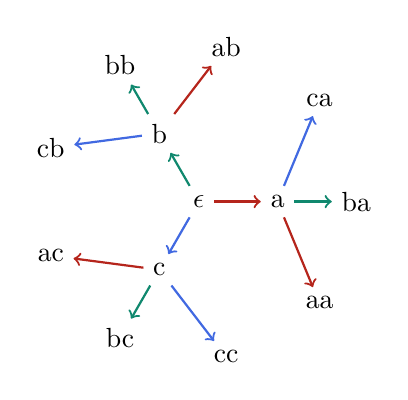
\begin{tikzpicture}
        \node (e) at (0,0) {$\epsilon$};
        \node (a) at (0:1) {a};
        \node (b) at (120:1) {b};
        \node (c) at (240:1) {c};
        \node (aa) at (-40:2) {aa};
        \node (ba) at (0:2) {ba};
        \node (ca) at (40:2) {ca};
        \node (ab) at (80:2) {ab};
        \node (bb) at (120:2) {bb};
        \node (cb) at (160:2) {cb};
        \node (ac) at (200:2) {ac};
        \node (bc) at (240:2) {bc};
        \node (cc) at (280:2) {cc};
    
        \draw[thick,->,BrickRed] (e) -- (a);
        \draw[thick,->,PineGreen] (e) -- (b);
        \draw[thick,->,RoyalBlue] (e) -- (c);
    
        \draw[thick,->,BrickRed] (a) -- (aa);
        \draw[thick,->,PineGreen] (a) -- (ba);
        \draw[thick,->,RoyalBlue] (a) -- (ca);
    
        \draw[thick,->,BrickRed] (b) -- (ab);
        \draw[thick,->,PineGreen] (b) -- (bb);
        \draw[thick,->,RoyalBlue] (b) -- (cb);
    
        \draw[thick,->,BrickRed] (c) -- (ac);
        \draw[thick,->,PineGreen] (c) -- (bc);
        \draw[thick,->,RoyalBlue] (c) -- (cc);
    \end{tikzpicture}
\end{center}
This is another algebra, with one nullary operator 
$\epsilon$ and three unary operators {\color{BrickRed}a$\Box$}, 
{\color{PineGreen}b$\Box$}, and {\color{RoyalBlue}c$\Box$}
being the production rules, that is the tree colors of arrows.

\code{Char:=['a','b',...,'z']}.
\begin{lstlisting}[language=Hidris]
data String = Empty | Prepend( head:Char, tail:String) 
\end{lstlisting}
Writing \lstinline{head:Char} or \lstinline{tail:String} 
indicates that head must come from the alphabet we chose 
and tail must be some already produced string, possibly empty.
Some readers might relate to a different dialect of 
programming such as the following
\begin{lstlisting}[language=Sava]
class String
    case Empty extends String
    case Prepend( head:Char, tail:String) extends String
sealed
\end{lstlisting}
The head here caries around what we put in the list and the tail 
is what comes next in the list.  Observe the similarities:
\begin{align}
     2 & \defeq S(S(0)) \tag{$\mathbb{N}$}\\
 \text{\lstinline{"me"}} & \defeq \text{\lstinline{Prepend('m',Prepend('e',Empty))}}
\tag{String}
\end{align}
The left-hand sides are merely notation for what the data really is on the right.
Both the successor and the \lstinline{Prepend} are operators that generate 
new values.  So part of algebra is to generate new data; so, it is no wonder 
that it closely connections to computation.



